\chapter*{Título do Apêndice 2}

\section*{Primeira seção do apêndice 2}

\par Neste apêndice é mostrado \ldots de acordo com a Figura~\ref{fig:ap2:identificador} é ilustrada a primeira tela deste processo.
\captionsetup[figure]{list=no}
\begin{figure}[h!]
 \centerline{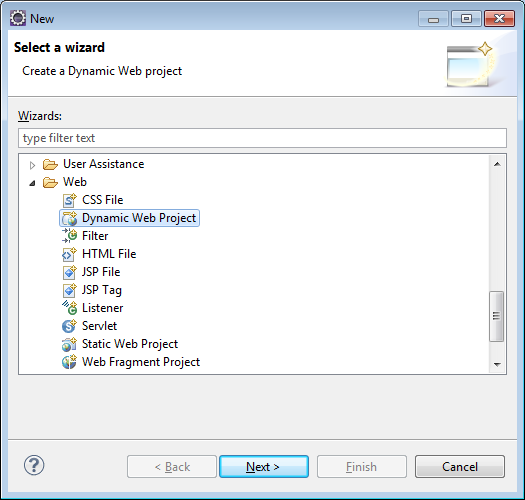
\includegraphics[scale=0.3]{./imagens/apendice_img1.png}}
 \caption[Outra imagem ainda.]
           {Outra imagem ainda. \textbf{Fonte:} Elaborado pelos autores}
  \label{fig:ap2:identificador}
\end{figure}

\section*{Segunda seção do apêndice 2}


\par Continuando \ldots na figura Figura~\ref{fig:xml_exemplo} é mostrado um exemplo de XML.

\begin{figure}[h!]
\begin{lstlisting}[style=custom_XML]
<project>
...
 <dependencies>
  ...
  <dependency>
   <groupId>org.neo4j</groupId>
   <artifactId>neo4j</artifactId>
   <version>1.9.4</version>
  </dependency>
  ...
 </dependencies>
 ...
</project>
\end{lstlisting}  
 \caption[Exemplo de código XML.]
           {Exemplo de código XML. \textbf{Fonte:} Elaborado pelos autores}
  \label{fig:xml_exemplo}
\end{figure}


